\section{Umsetzung der Kollisionsvermeidung} \label{sec:durchführung}

Dieser Abschnitt gliedert sich in vier Unterabschnitte. Der erste beschäftigt sich damit, wie aus einem Jupyter Notbook (in der Programmiersprache Python) der Jetbot \bzw dessen Motoren angesteuert werden können, so dass sich dieser bewegt. Darauf folgt im nächsten Unterabschnitt das sammeln von Daten, konkret Bildern, um das CNN später zu trainieren. Mittels dieser Trainingsdaten wird im nächsten Unterabschnitt ein Modell angelernt mittels Transfer-Learning, welches im letzten Unterabschnitt in einer Live-Demo Anwendung findet.\\

Alle aufgezeigten Inhalte finden sich in Code-Form dokumentiert im Anhang wieder und können dort im Detail nachvollzogen werden.

\subsection{Ansteuern des Jetbot Roboters} \label{sec:steuern-robot}

Um mit der Programmierung des Jetbots zu beginnen, muss zunächst die von der Nvidia-Jetbot-Community bereitgestellte Klasse \glqq\texttt{Robot}\grqq{} importiert werden. Diese ist Teil des Jetbot-Package, welches in Python eingebunden werden kann. Dies ist bereits geschehen, da für sie Inbetriebnahme (siehe \autoref{sec:versuchsaufbau}) ein vorkonfiguriertes Image verwendet wurde. Mit der Klasse können die Motoren des Roboters angesteuert werden. \\
Eine hilfreiche Ergänzung sind die sogenannten \glqq traitlets\grqq{}, über welche es möglich ist Widgets zu implementieren, mit denen man in einer grafischen Oberfläche im Browser den Jetbot Roboter steuern kann. Über diese ist es auch möglich Funktionen mit Events zu verknüpfen. So kann dann \zB über einen Button-Druck eine Vorwärtsbewegung ausgelöst werden.\\

\begin{figure}[H]
    \centering
    \begin{subfigure}{0.253\textwidth}
        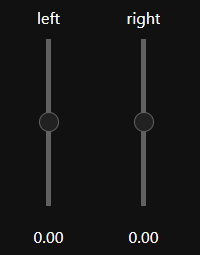
\includegraphics[width=1.0\linewidth]{Bilder/slider.png}
        \caption{Slider Steuerung}
    \end{subfigure}
    \begin{subfigure}{0.5\textwidth}
        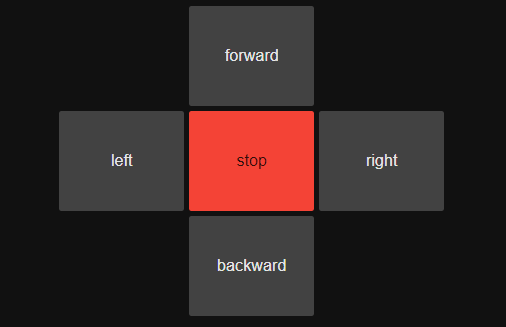
\includegraphics[width=1.0\linewidth]{Bilder/buttons.png}
        \caption{Button Steuerung}
    \end{subfigure}
    \label{fig:Bild4.1}
    \caption[Widget-Steuerung]{Widgets zum Steuern des Jetbots mithilfe von traitlets}
\end{figure}

Eine dritte grundlegende Funktion ist der \glqq Killswitch\grqq{}. Dabei handelt es sich konkret um eine Sicherheitsfunktion, die dafür sorgt, dass der Roboter in seiner Bewegung stoppt, wenn er die Verbindung zur JupyterLab Web-Oberfläche verliert.

\subsection{Aufnehmen von Trainingsdaten}

Nun wo die Möglichkeit besteht den Roboter per Code manuell zu fahren, ist der nächste Schritt, dass dieser sich von alleine ohne menschliches Einwirken fortbewegen kann. Schwierig ist dabei die Anforderung, dass sämtliche Bewegungen kollisionsfrei stattfinden sollen. Dazu muss der Jetbot \bzw dessen CNN mit Trainingsdaten angelernt werden. Damit der Roboter in mehreren Epochen effektiv trainiert werden kann müssen diese Daten zunächst aufgenommen werden.\\
Der Ansatz für das kollisionsfreie Bewegen ist in seinem Konzept sehr simpel. Ziel ist es eine virtuelle \glqq Safety Bubble\grqq{} um den Roboter zu erstellen. In dieser kann der Jetbot sich frei im Kreis drehen, ohne dass er mit Objekten kollidiert oder von einem Vorsprung herunterfällt. Nicht berücksichtigt wird in diesem Ansatz, dass sich natürlich auch Objekte außerhalb des Sichtfeldes in die sichere Zone hinein bewegen können. Er kann sich also ausschließlich nicht von selbst durch seine eigenen Bewegungen in eine \glqq gefährliche Situation\grqq{} begeben.\\
Konkret umgesetzt wird der Ansatz über den einzigen aber höchst effektiven Sensor des Roboters, die Weitwinkelkamera. Zunächst wird der Roboter manuell in Szenarien platziert, in denen seine Sicherheitsblase verletzt wird. Diese werden als \glqq\texttt{blocked}\grqq{} gelabelt. Dazu wird ein Bild gespeichert von dem, was der Roboter sieht, zusammen mit dem Label.\\
Zweitens wird der Roboter manuell in Szenarien platziert, in denen es sicher ist sich ein Stück vorwärts zu bewegen. Diese Szenarien werden als \glqq\texttt{free}\grqq{} gelabelt. Ebenfalls wird ein Bild zusammen mit dem Label abgespeichert.\\
Nachdem genügen Trainingsdaten aufgenommen wurden, können diese auf einen mit einer GPU ausgestatteten Rechner geladen werden, wo das neuronale Netzwerk trainiert wird vorherzusagen, ob die Sicherheitsblase des Roboters verletzt wurde anhand der Live-Bilder, die dieser aufnimmt.

\begin{figure}[H]
    \centering
    \fbox{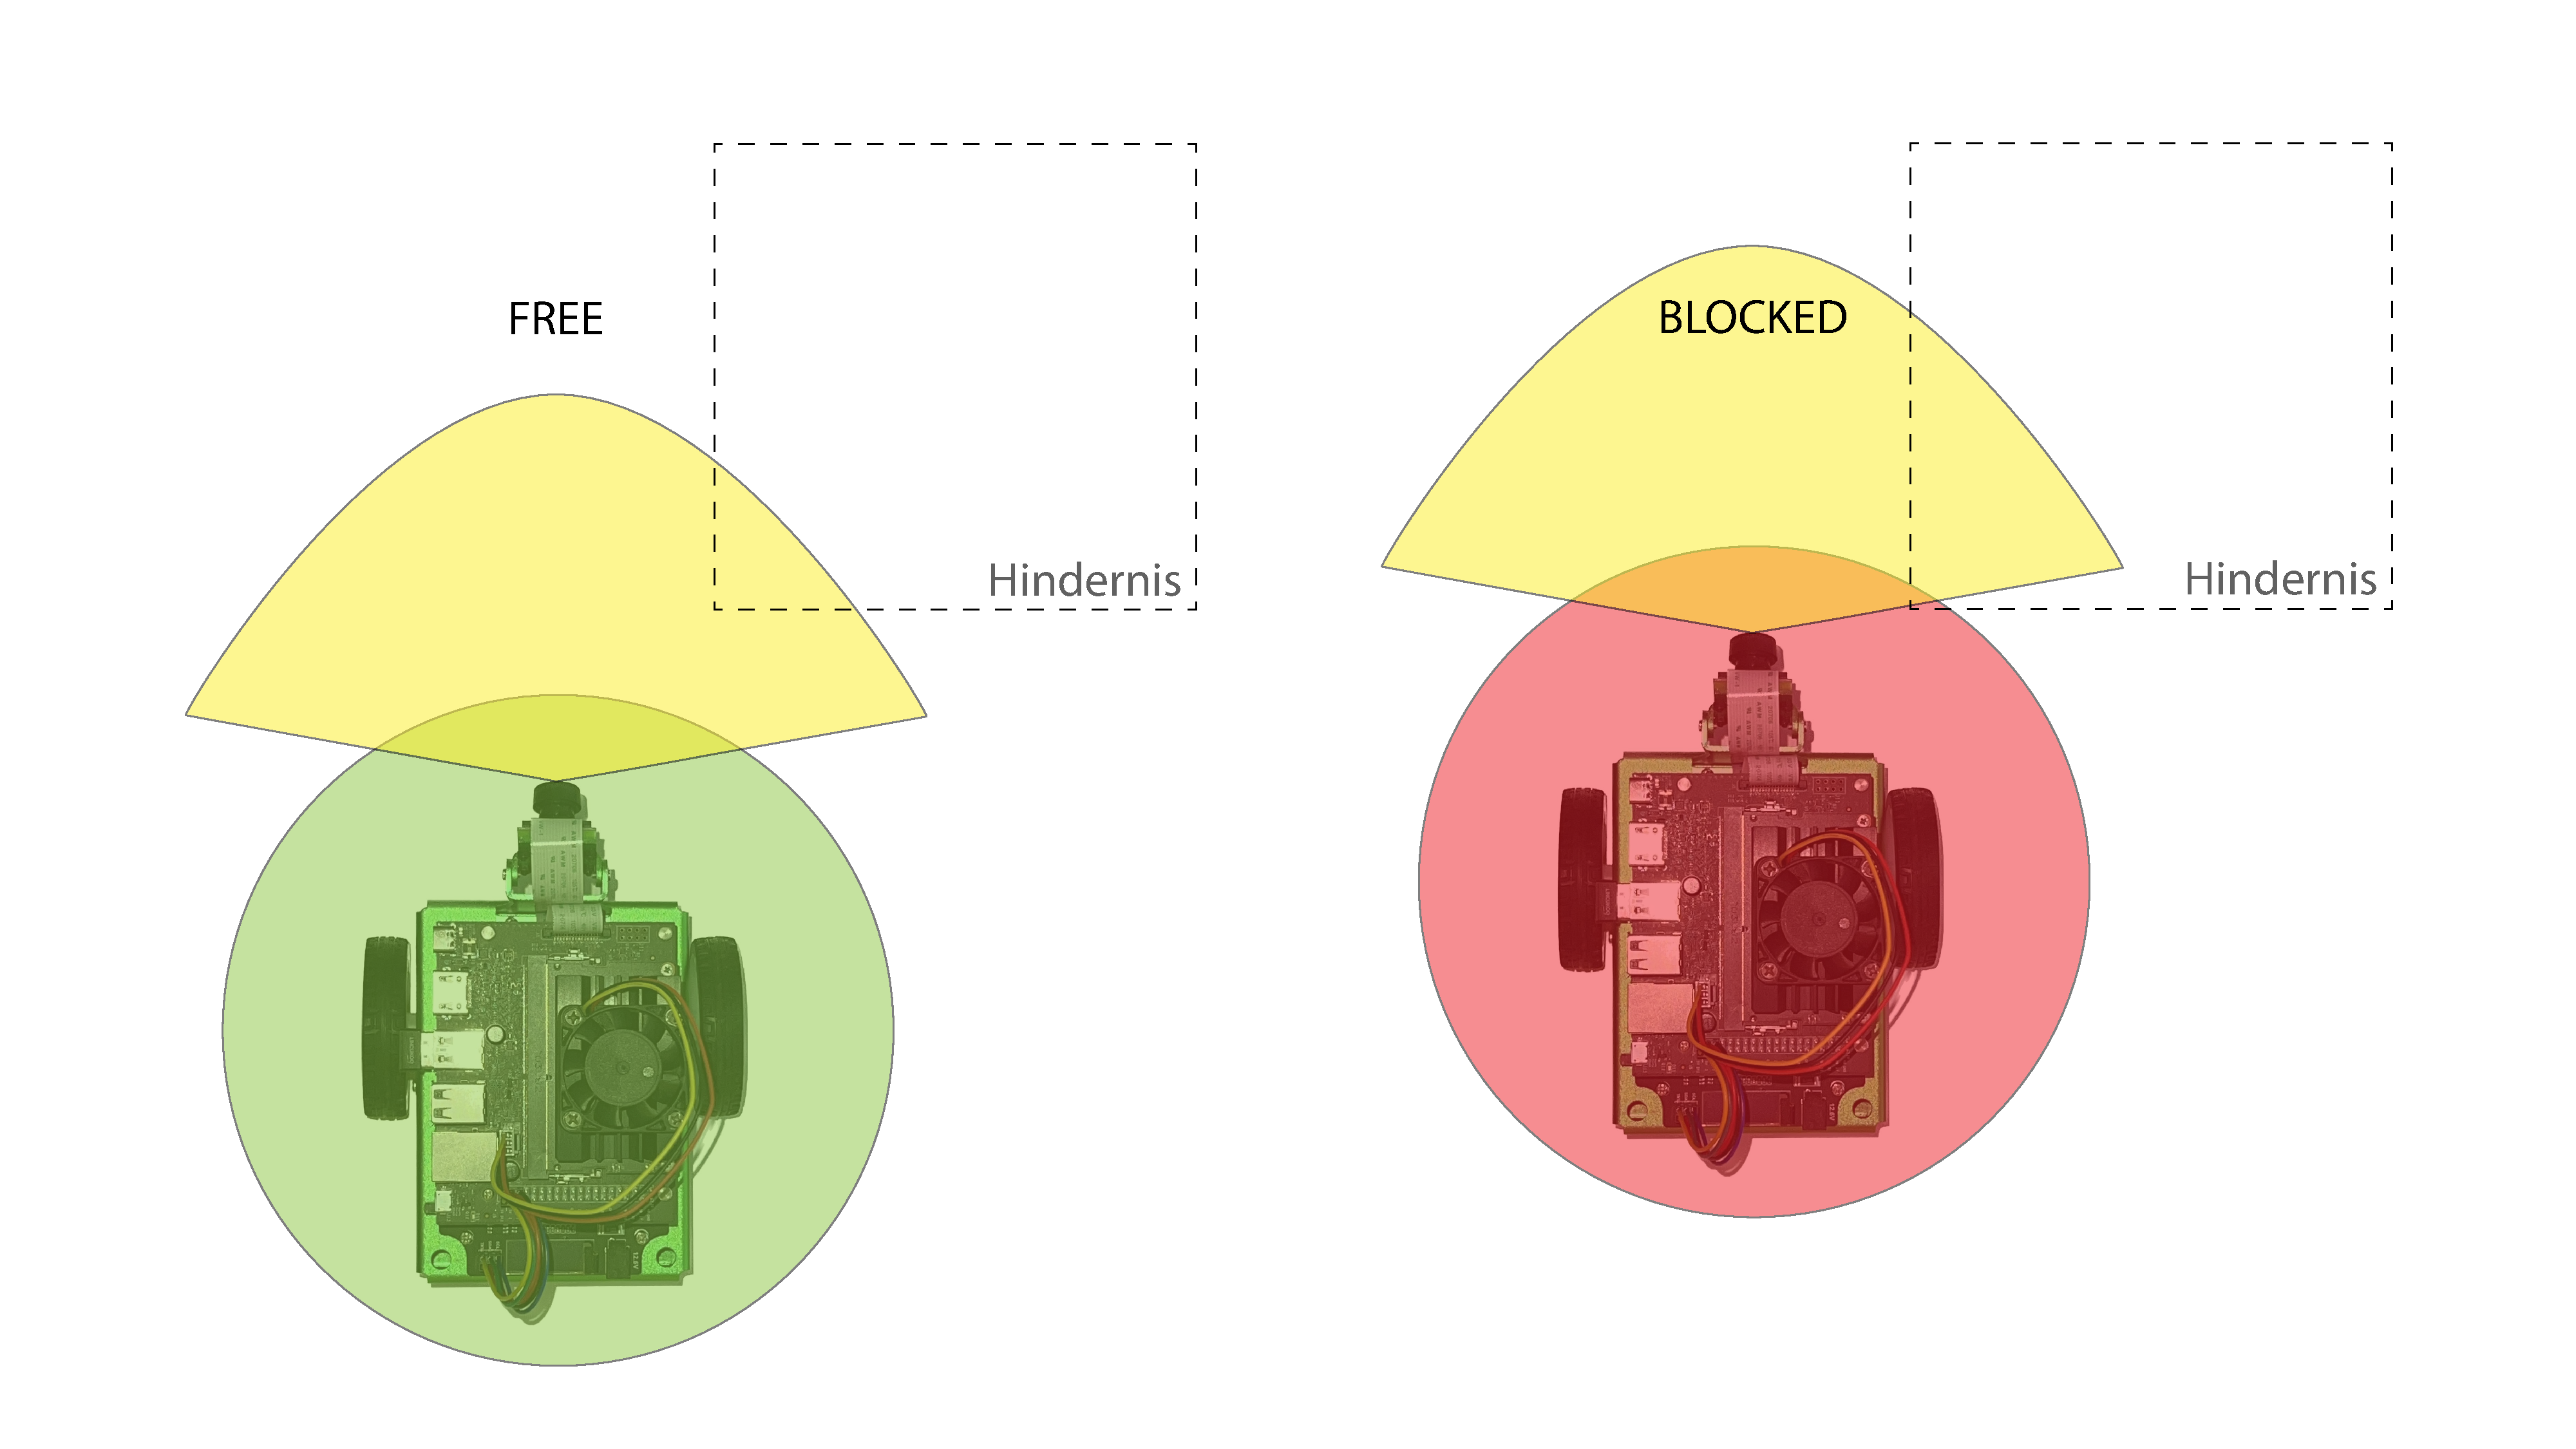
\includegraphics[width=0.98\textwidth]{Bilder/Safety-Bubble.pdf}}
    \caption[Safety Bubble des Jetbot]{Sicherheitsblase des Jetbot Roboterfahrzeugs im \texttt{free} und \texttt{blocked} Szenario}
    \label{fig:Bild4.2}
\end{figure}

\subsection{Pre-Training des CNN AlexNet}

Im nächsten Schritt wird das neuronale Netz trainiert, so dass ein möglichst ideales Modell erstellt werden kann, welches im realen Betrieb des Roboters Einsatz findet. Für das Trainieren des Modells wird die Python Bibliothek PyTorch verwendet. Dabei handelt es sich um eine Sammlung von Funktionen und Klassen, die für \glqq Deep Learning\grqq{} entwickelt wurden. \\
Zunächst werden die in zwei Klassen unterteilten Bilder auf einen Rechner transferiert, welcher über einen Grafikprozessor (GPU) verfügt. Das könnte zum einen der Jetbot selbst sein oder ein separater Computer. Je nach gewähltem CNN und dessen Anzahl an Layern ergibt es jedoch Sinn, einen Leistungsstarken Computer mit einer schnellen Grafikkarte zu verwenden. Wie bereits Eingangs erwähnt wurde, soll das CNN AlexNet verwendet werden, welches moderate Anforderungen an die Rechenleistung stellt. Somit ist es grundsätzlich möglich bei kleiner Anzahl an Epochen (\zB 30 Epochen) das Trainieren auf dem Jetson Nano Mikrocontroller selbst durchzuführen. \\
Bevor die Bilddaten in Kombination mit dem AlexNet verwendet werden können, müssen diese an dessen Vorgaben angepasst werden. Dazu zählt zum einen die Anpassung der Bildgröße auf eine Auflösung von 224x224 Pixeln, zum anderen das Umwandeln der Daten in Tensoren, welche im gleichen Schritt normalisiert werden. Ein Tensor meint dabei eine Anordnung von Zahlen entlang $n$ Achsen. Die Zahl $n$ heißt die Stufe des Tensors. \\
Als Nächstes wird der Datensatz in einen Trainings- und einen Testsatz aufgeteilt. Der Testdatensatz wird verwendet, um die Genauigkeit des trainierten Modells zu überprüfen.\\
Nachdem alle Vorbereitungen getroffen wurden, kann nun das eigentliche neuronale Netz definiert werden. Das \glqq torchvision\grqq{} Paket (aus der PyTorch Bibliothek) bietet bereits eine Sammlung von vortrainierten Modellen, von welchen das AlexNet ausgewählt wurde. Dieses Modell, welches bereits mit Millionen von Bildern trainiert wurde, kann mit Hilfe des Transfer Learning aus \autoref{sec: transfer-learning} auf den kleinen Datensatz an Bildern angewendet werden, der im vorherigen Unterabschnitt aufgenommen wurde. Wichtige Merkmale, die beim ursprünglichen Training des vortrainierten Modells gelernt wurden, können damit für die neue Aufgabe (das kollisionsfreie Fahren) wiederverwendet werden. \\
Das CNN wird in 30 Epochen trainiert, wobei aus jeder Epoche das Modell mit der besten Leistung abgespeichert wird. Pro Epoche wird einmal der komplette Datensatz an Bildern durchgearbeitet. \\
Nach Beendigung aller Epochen wurde ein möglichst optimales Modell errechnet, welches im nächsten Unterabschnitt im Live-Betrieb eingesetzt wird.

\subsection{Live-Demo des trainierten CNN}

Im letzten Unterabschnitt der Umsetzung wird das trainierte Modell eingesetzt, um dem Jetbot die Fähigkeit zu geben zu erkennen, ob ein Szenario als \texttt{free} oder \texttt{blocked} bewertet werden muss, so dass beim Fahren sämtliche Kollisionen vermieden werden können. \\
Dazu wird das Modell auf den Jetson Nano geladen. Im nächsten Schritt muss dafür gesorgt werden, dass die Live-Kameradaten wie bereits die Trainingsbilder an die Anforderungen des AlexNet angepasst werden. Dieser Prozess wird als Vorverarbeitung (engl.\xspace Preprocessing) bezeichnet. Dabei werden über das Python Paket opcenCV die Bilddaten von \texttt{BGR} zu \texttt{RGB} konvertiert, die Daten normalisiert und dann von der CPU auf die GPU transferiert. Die Umsetzung des Preprocessing erfolgt in einer Funktion, die später aufgerufen werden kann, wenn ein neues Bild verarbeitet werden muss. \\
Weiterhin muss wie auch schon in \autoref{sec:steuern-robot} die Roboter-Klasse importiert werden, so dass die Motoren des Jetbots angesteuert werden können.\\
Ist dies geschehen kann die Funktion \glqq\texttt{update}\grqq{} implementiert werden, welche jedes mal aufgerufen wird, wenn die Kamera ein neues Bild aufnimmt. In dieser werden drei Aufgaben der Reihe nach ausgeführt:

\begin{enumerate}
    \item Vorverarbeitung des Kamerabildes
    \item Ausführung des neuronalen Netzes
    \item Wenn das CNN \texttt{blocked} ausgibt, nach links fahren,\\
    und wenn es \texttt{free} ausgibt, dann vorwärts fahren.
\end{enumerate}

Der letzte Schritt ist es diese Funktion mit der Weitwinkelkamera zu verbinden. Dazu wird eine \texttt{observe}-Funktion (Beobachter-Funktion) mit dem Value-traitlet (siehe \autoref{sec:steuern-robot} der Kamera verbunden, welche dann die \texttt{update}-Funktion aufruft, wenn der Value (Wert) der Kamera eine Änderung erfährt.

\begin{figure}[H]
    \centering
    \begin{subfigure}{0.45\textwidth}
        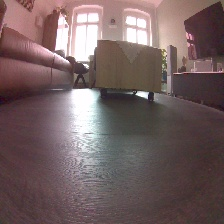
\includegraphics[width=0.9\linewidth]{Bilder/live-demo.jpg}
    \end{subfigure}
    \begin{subfigure}{0.45\textwidth}
        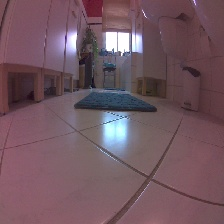
\includegraphics[width=0.9\linewidth]{Bilder/live-demo2.jpg}
    \end{subfigure}
    \label{fig:Bild4.3}
    \caption[Live Demo Jetbot]{Kamera Aufnahmen des Jetbots während des kollisionsfreien Fahrens}
\end{figure}

Der Jetbot kann nach bedarf wieder gestoppt werden über einen \texttt{unobserve}-Aufruf und die Stopp-Routine der Roboterklasse. Alle implementierten Programme und Funktionen können im Anhang nachgelesen werden. Dort befinden sich sämtliche Jupyter Notebooks.